%% This is file `elsarticle-template-1-num.tex',
%%
%% Copyright 2009 Elsevier Ltd
%%
%% This file is part of the 'Elsarticle Bundle'.
%% ---------------------------------------------
%%
%% It may be distributed under the conditions of the LaTeX Project Public
%% License, either version 1.2 of this license or (at your option) any
%% later version.  The latest version of this license is in
%%    http://www.latex-project.org/lppl.txt
%% and version 1.2 or later is part of all distributions of LaTeX
%% version 1999/12/01 or later.
%%
%% The list of all files belonging to the 'Elsarticle Bundle' is
%% given in the file `manifest.txt'.
%%
%% Template article for Elsevier's document class `elsarticle'
%% with numbered style bibliographic references
%%
%% $Id: elsarticle-template-1-num.tex 149 2009-10-08 05:01:15Z rishi $
%% $URL: http://lenova.river-valley.com/svn/elsbst/trunk/elsarticle-template-1-num.tex $
%%
% \documentclass[preprint,12pt]{elsarticle}

%% Use the option review to obtain double line spacing
%% \documentclass[preprint,review,12pt]{elsarticle}

%% Use the options 1p,twocolumn; 3p; 3p,twocolumn; 5p; or 5p,twocolumn
%% for a journal layout:
%% \documentclass[final,1p,times]{elsarticle}
%% \documentclass[final,1p,times,twocolumn]{elsarticle}
%  \documentclass[final,3p,times]{elsarticle}
 \documentclass[final,3p,times,twocolumn]{elsarticle}
%% \documentclass[final,5p,times]{elsarticle}
%% \documentclass[final,5p,times,twocolumn]{elsarticle}

%% if you use PostScript figures in your article
%% use the graphics package for simple commands
%% \usepackage{graphics}
%% or use the graphicx package for more complicated commands
%% \usepackage{graphicx}
%% or use the epsfig package if you prefer to use the old commands
%% \usepackage{epsfig}

\usepackage[utf8]{inputenc} 
%% The amssymb package provides various useful mathematical symbols
\usepackage{amssymb}
\usepackage{hyperref}
\usepackage{graphicx}
\usepackage{subcaption}
\usepackage{lscape}
\usepackage{amsmath}
\usepackage{multirow}
% if you have landscape tables
\usepackage[figuresright]{rotating}
\usepackage{lineno}
\usepackage{algorithm} 
\usepackage{algpseudocode} 
\usepackage{comment}
\usepackage{lineno}

\usepackage{natbib}
\bibliographystyle{abbrvnat}
\setcitestyle{authoryear,open={(},close={)},citesep={;}} 

\usepackage{calc}
\setlength{\footskip}{\paperheight
  -(1in+\voffset+\topmargin+\headheight+\headsep+\textheight)
  -0.95in}

% for SVG figures
\usepackage{svg}

% For using LuaLaTeX or XeLaTeX compilers instead of pdflatex (memory limit)
\usepackage{fontspec} 
\setmainfont{Times New Roman}

\usepackage{titlesec}
\titleformat{\section}{\normalfont\bfseries}{\thesection}{1em}{}
\titleformat{\subsection}{\normalfont\itshape}{\thesubsection}{1em}{}

% Placeholder for numbers that come from runs still in progress. Fill from
%   python scripts/aggregate_results.py --latex      (tables)
%   python scripts/benchmark_efficiency.py           (latency)
% and delete this macro once no \tbd remains.
\newcommand{\tbd}{\textemdash}


\begin{document}

\begin{frontmatter}

\title{Confidence Aware Deep Learning for Invasive Aquatic Plant Identification}


\author[label1]{Aaryan Panigrahi}
\author[label1]{Yaman}
\author[label1]{Fengying Dang}


\address{Fengying Dang (fdang1@mtu.edu) is the corresponding author}
\address[label1]{Department of Electrical and Computer Engineering, Michigan Technological University, Houghton, MI 49931, USA}


\begin{abstract}
Aquatic invasive species threaten fisheries and aquaculture through ecological damage and economic losses. Although deep learning has advanced image classification, conventional classifiers typically produce predictions from a single analysis of each image, which may be insufficient to distinguish invasive plants from morphologically similar native species. To address this challenge, we propose a confidence-aware classification framework incorporating a You Need to Look Twice (YNLT) module into a ConvNeXt-V2 Tiny architecture with a classification head. YNLT selectively re-examines images using multi-scale patches when prediction confidence, the margin between the top two class scores, and predictive entropy indicate potential misclassification. We evaluate the framework on a dataset of 1,030 photographs covering 21 aquatic plant species, including five invasive species. The proposed architecture achieves a top-1 accuracy of 58.6--59.5\% in the systematic evaluation. Fine-tuning the final ConvNeXt stage while keeping earlier stages frozen increases pooled accuracy to \(65.1\% \pm 5.0\%\). More importantly, integrating YNLT with the gated-attention head reduces the invasive species false negative rate (FNR) from \(32.6\% \pm 3.9\%\) to \(17.4\% \pm 5.7\%\), while changing pooled accuracy by less than one percentage point. Gradient-weighted class activation mapping and species-level error analysis further reveal that residual classification errors are concentrated among morphologically similar pondweeds. These results demonstrate the potential of confidence-aware image re-evaluation to improve invasive aquatic plant identification, particularly when reducing missed detections is more important than maximizing overall classification accuracy.
\end{abstract}

\begin{keyword}
Aquatic invasive species \sep Computer vision \sep Fine-grained recognition \sep Environmental monitoring
\end{keyword}

\end{frontmatter}

%%%%%%%%%%%%%%%%%%%%%%%%%%%%%%%%%%%%%%%%%%%%%%%%%%%%%%%%%%%%%%%%%%%%%%%%%%%%%%%%%%%%%%%%%%%%%%%%%%%%%%%%%%%%%%%%%%%%%%%%%%%%%%%%%%%%%%
%% main text
\section{Introduction}
\label{sec:intro}

Invasive species threaten biosecurity, agriculture, and human health, with global control and damage costs estimated in the trillions of dollars~\citep{tasker2024nuanced, macedo2024economic, shen2024typical, vaissiere2022nature, cuthbert2021global}. In the United States, recent estimates place annual losses near \$138 billion, a large fraction of which is attributable to freshwater plants, especially submerged and floating taxa~\citep{pimentel2000environmental, lovell2006economic, warziniack2021economics, macedo2024economic}.In fisheries and aquaculture, dense growth of invasive aquatic plants can deplete dissolved oxygen, disrupt spawning habitats, obstruct equipment, and increase operational costs. Early and accurate identification is therefore essential for effective monitoring and management.

Existing identification methods do not scale to routine monitoring. Field identification depends on botanical expertise~\citep{dehez2023investigation}. Molecular assays are accurate but require specialized sampling and laboratory capacity~\citep{angles2019detection, ghahramanzadeh2013efficient, scriver2015development}. Remote sensing covers large areas but lacks the spatial detail needed to separate morphologically similar floating species and not working on submerged ones~\citep{brooks2019implementing, unitis2018remote, jochems4883509active}. Image-based computer vision provides a possibility to achieve good identification of the aquatic plants~\citep{wang2026realtime}. However, aquatic plants images are limited accessible due to the difficulties of collecting them. 

Prior studies have demonstrated the effectiveness of convolutional neural networks for aquatic plant classification, including seagrass classification~\citep{DeepSeaGrass1, Nawaz2025Seagrass, Paul2023LWDS, baos_cnn}, kelp classification from autonomous-underwater-vehicle images~\citep{mahmood2020kelp}, macroalgae identification from underwater photographs~\citep{sonmez2026macroalgae}, and citizen science based plant identification~\citep{joly2016plantnet}. However, identifying invasive aquatic plants presents additional challenges because closely related native and invasive species may share similar morphological characteristics, while labeled photographs can be limited. Transfer learning from models pretrained on large datasets can help mitigate the challenges associated with limited labeled data.~\citep{Kelps_SVMs}. However, distinguishing morphologically similar species remains challenging when photographs vary in background, scale, and viewing angle.

Several computer vision approaches have explored how additional detailed visual information can improve fine-grained recognition. Recurrent attention models use sequential glimpses, often guided by reinforcement learning, to focus on informative image regions~\citep{mnih2014recurrent}. Coarse-to-fine and recurrent attention CNNs learn to identify discriminative regions at different levels of detail~\citep{fu2017look}. Multi-resolution networks and multi-crop test-time augmentation aggregate predictions from multiple scales or image crops, potentially increasing inference cost because additional views are processed for each image~\citep{krizhevsky2012imagenet, huang2018multiscale}. Attention-based fine-grained recognition methods emphasize discriminative object parts, while hard-example mining focuses on difficult samples during training~\citep{fu2017look, shrivastava2016training}. Complementary work on uncertainty estimation and selective prediction addresses prediction reliability through calibration~\citep{Guoetal2017, Ovadiaetal2019, hendrycks2017baseline} or allows models to abstain when confidence is insufficient~\citep{geifman2017selective}. 

To address these challenges, we propose a confidence-aware classification framework incorporating a You Need to Look Twice (YNLT) module into a ConvNeXt-V2 Tiny architecture with a classification head. In contrast to previous approaches, this method uses prediction confidence, the margin between the top two class scores, and predictive entropy to determine whether an image requires further analysis through multi-scale patches. Rather than applying additional processing to every image or abstaining from uncertain predictions, YNLT selectively re-examines potentially misclassified images while retaining the goal of assigning a species label. This strategy is particularly relevant to invasive aquatic plant identification, where limited labeled data, morphological similarity, and the consequences of missed detections motivate more targeted image analysis. ConvNeXt-V2 Tiny~\citep{liu2022convnet, Wooetal2023} is chosen as the backbone with the intention of future onboard running on marine robot. The major contributions of this paper
are highlighted as follows:
\begin{enumerate}
\item A diverse dataset consisting of 1{,}030 images of 21 aquatic species with five invasive species important to fresh water in the northern U.S.;

\item A confidence-aware re-evaluation module, You Need to Look Twice (YNLT), that selectively applies multi-scale patch analysis to images with potentially unreliable predictions, as indicated by prediction confidence, the margin between the top two class scores, and predictive entropy.

\item A systematic evaluation of classification performance and error patterns, comparing linear, multilayer perceptron, and gated-attention heads with a frozen ConvNeXt-V2 Tiny encoder and assessing the effect of fine-tuning the final encoder stage. Learning curves, Grad-CAM visualizations~\citep{selvaraju2017gradcam}, and species-level error analysis further characterize the effects of training sample size and morphological similarity on classification performance.
\end{enumerate}

The remainder of the paper is organized as follows. Materials and methods are presented in Section~\ref{sec:materials_methods}. Results are reported in Section~\ref{sec:results}. Limitations and computational cost are discussed before the conclusions in Section~\ref{sec:conclu}.

\section{Materials and Methods}
\label{sec:materials_methods}

\subsection{Study area}
\label{subsec:study_area}

The geographic focus of this study is the state of Michigan, which encompasses portions of four Great Lakes (Lake Superior, Lake Michigan, Lake Huron, and Lake Erie) alongside numerous smaller inland lakes. These freshwater systems support highly diverse ecological communities, including a wide variety of native aquatic plant and fish species. However, the balance of these habitats is increasingly threatened by the introduction and proliferation of aquatic invasive plants. The classification task in this paper is limited to 21 aquatic plant species that occur in these waters, five of them invasive and sixteen native. Figure \ref{fig:map} shows where the study is focused and the approximate locations at which those 21 species have been recorded.

\begin{figure*}[!h]
\centering
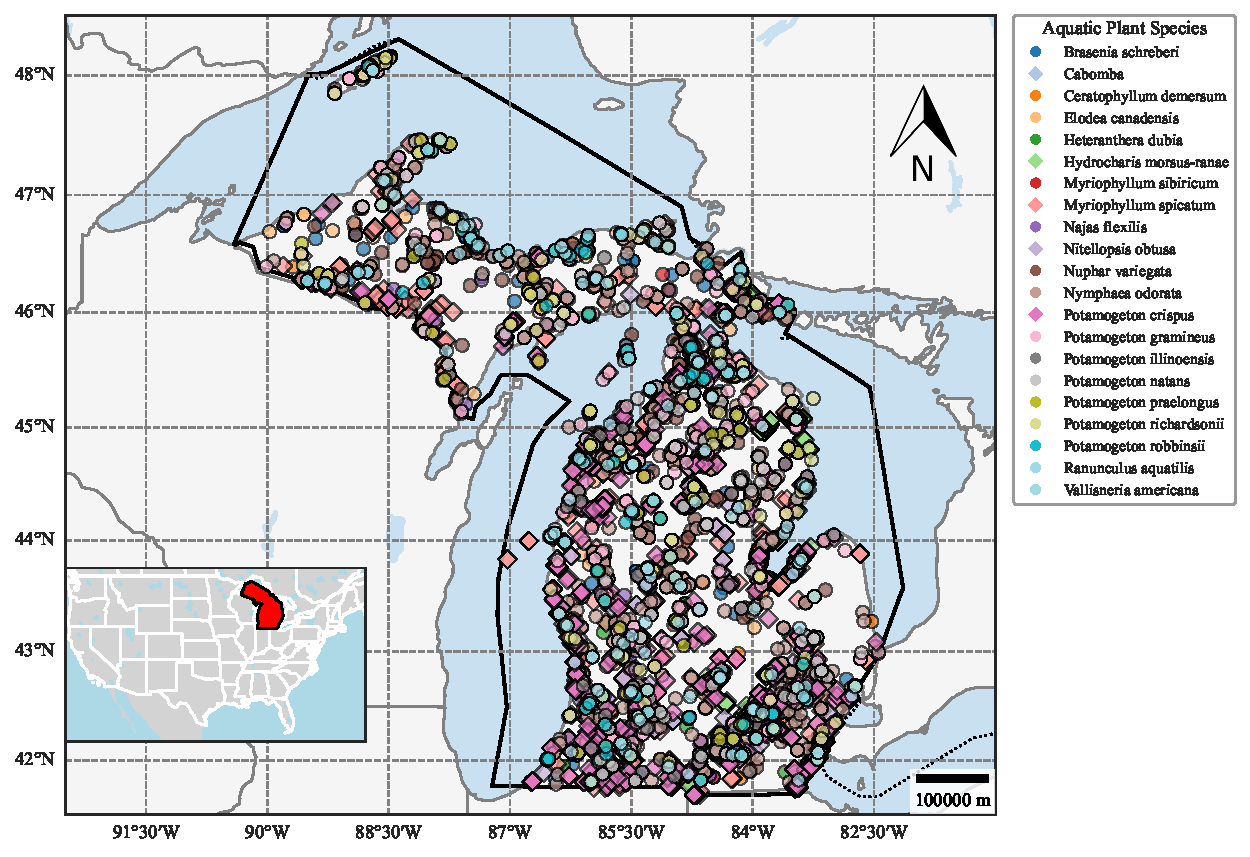
\includegraphics[width=1.0\textwidth]{figs/map.pdf}
\caption{Geographic focus of the study: the 21 Michigan aquatic plant species classified in this paper. Points are approximate occurrence records from the Global Biodiversity Information Facility (GBIF). Diamond markers are the five invasive species and circular markers are the 16 native species. The inset shows Michigan within the contiguous United States. Lakes Superior, Michigan, Huron, and Erie border the state.} 
\label{fig:map}
\end{figure*}

\subsection{Dataset details}
\label{subsec:dataset}
Data collection in underwater environments is difficult. This study therefore uses one mixed collection of the same 21 species (Figure~\ref{fig:data}). The collection is reported as 203 laboratory photographs and 827 outdoor photographs (1{,}030 in total). The outdoor total combines 785 openly licensed field photographs from biodiversity databases with 42 locally collected outdoor photographs. These photographs are pooled and split together. Handheld photographs, 307 images, are stored separately and are not used for training, validation, or testing.

\subsubsection{Laboratory photographs}
The laboratory source contains 203 photographs at \(1500\times 1000\) pixels. Several species have only two or three photographs. Basic preprocessing removed reference artifacts such as coins and scales where they could be cropped without removing the plant.

\subsubsection{Outdoor photographs}
\label{subsec:webdata}

Most of the outdoor photographs were obtained by querying GBIF for occurrence records of each of the 21 species and downloading the associated photographs~\citep{gbif2026}. The download was then reviewed. Duplicate photographs, photographs that did not show the named species, and handheld photographs were removed. After that review, 785 photographs remain from this source. An additional 42 locally collected outdoor photographs of 9 species (16 of them \emph{Nuphar variegata}) are included in the same outdoor total, bringing outdoor photographs to 827. In Figure~\ref{fig:data} these sources are not shown separately; both are counted as outdoor. \emph{Elodea canadensis} has no remaining outdoor photographs after cleaning, so that species is represented only by its 15 laboratory images. Every retained image is stored with its licence and rights holder. Records that do not permit redistribution are used for research only and are not released as a dataset.

A GBIF occurrence often carries several photographs of the same plant. Splitting by image would place photographs of one plant in both the training and test sets. Photographs that belong to one occurrence are therefore kept in a single split.

Because a 60/20/20 split leaves only about eight of the 42 locally collected outdoor photographs in a given test portion, accuracy on that small slice is not used to rank models.

\subsubsection{Splits}
Within each species, 60\% of the images are assigned to training, 20\% to validation, and 20\% to test. Observation-grouped photographs stay in one split. For seed 8 the pooled split is 655 training, 189 validation, and 186 test images. Other seeds move a few outdoor photographs between splits, so the pooled test contains 186 to 190 images. Split lists are stored as CSV files with the released code.

\begin{figure*}[!ht]
    \centering
    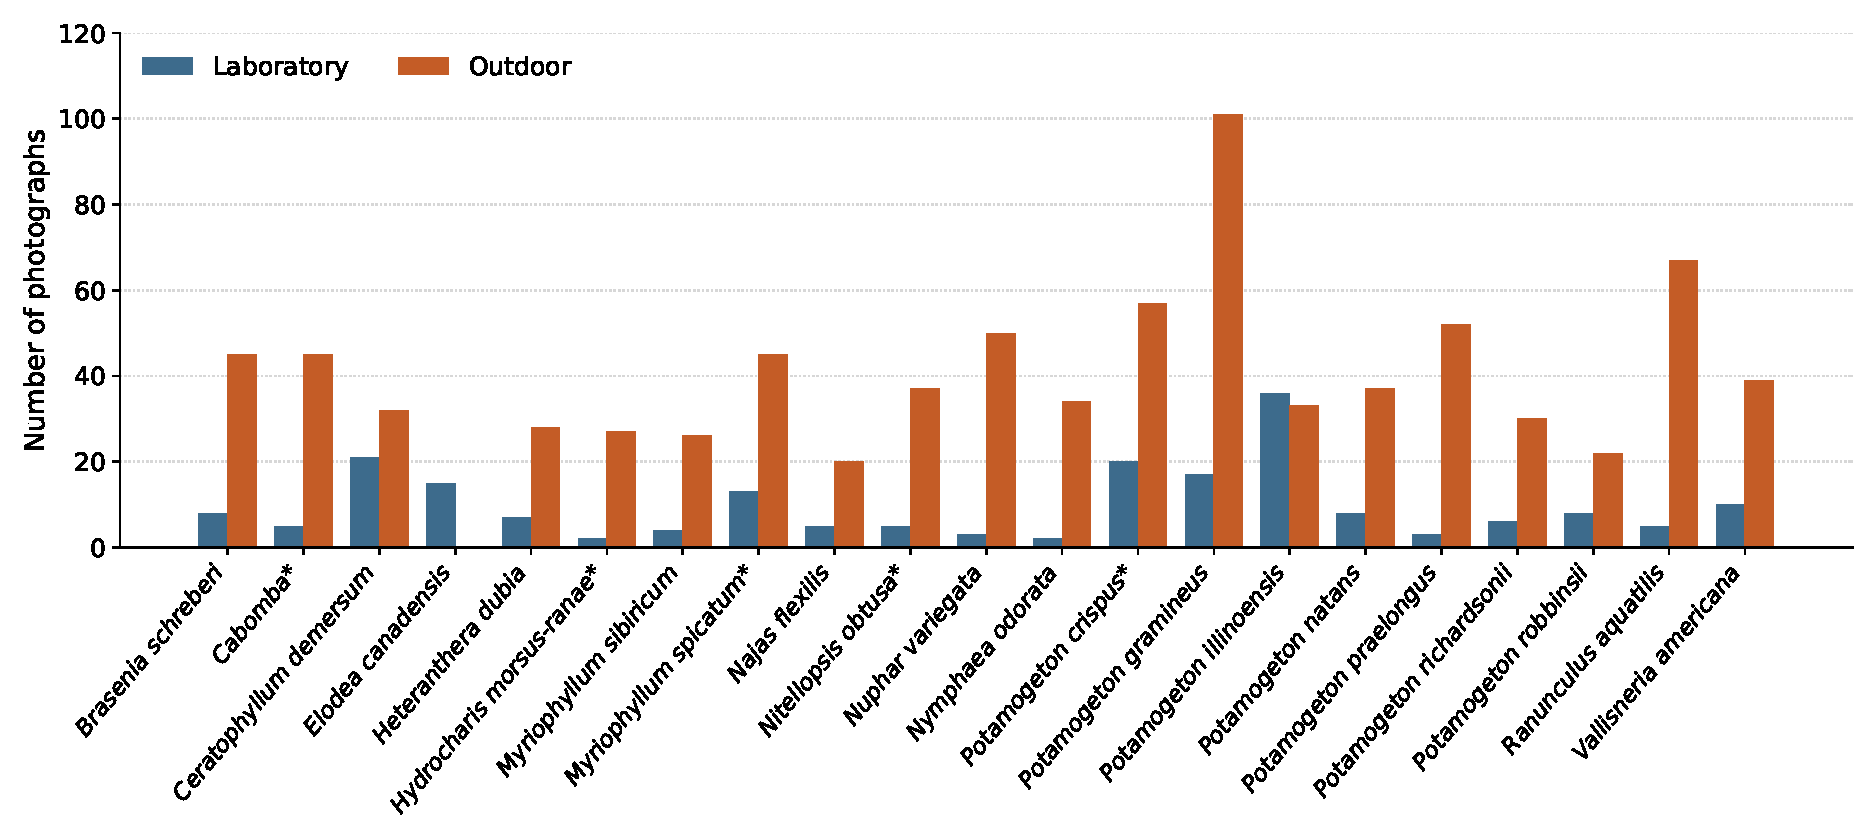
\includegraphics[width=1.0\textwidth]{figs/species_counts.pdf}
    \caption{Number of photographs of each of the 21 study species in the 1{,}030-image collection (203 laboratory and 827 outdoor). For each species the left bar is the laboratory count and the right bar is the outdoor count. Outdoor combines web-sourced field photographs and locally collected outdoor photographs. Asterisks mark the five invasive species. Handheld photographs are excluded. \emph{Elodea canadensis} has laboratory photographs only.}
    \label{fig:data}
\end{figure*}

\subsubsection{Preprocessing and Augmentation}

\begin{figure*}[!h]
\centering
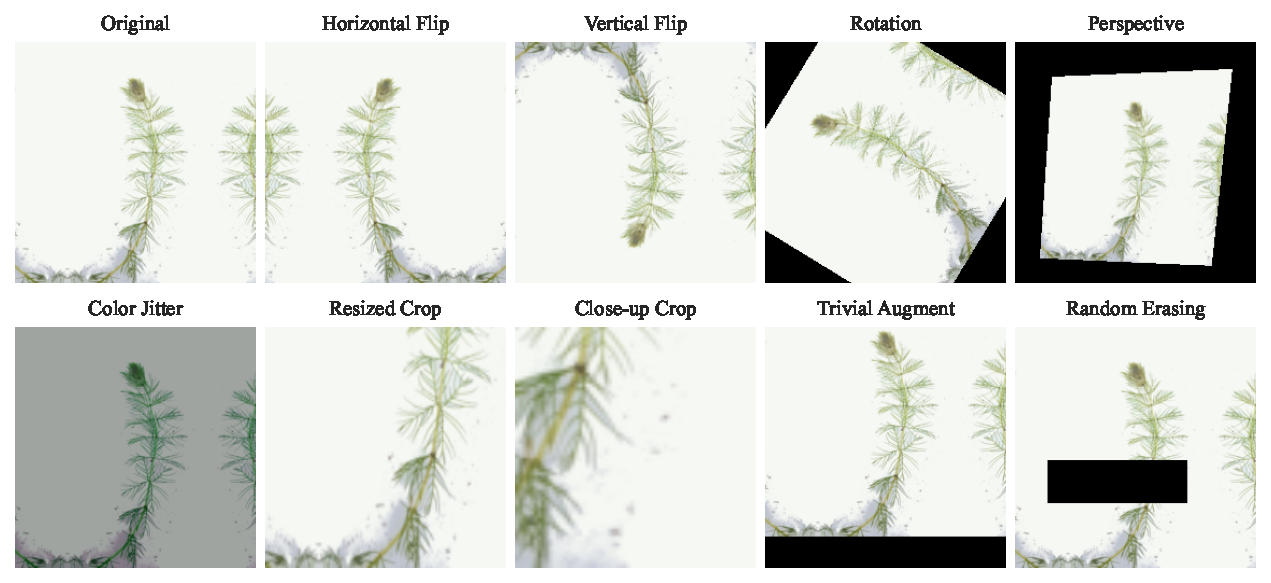
\includegraphics[width=0.9\textwidth]{figs/augmentations.pdf}
\caption{Various data augmentation techniques applied to the original images. The first row demonstrates basic geometric augmentations. The augmentations in the second row were specifically tuned to improve generalization from a small dataset. The close-up crop allows the model to learn from high-resolution details that would otherwise be lost during downsampling.} 
\label{fig:augmentations}
\end{figure*}

Given a training split of a few hundred images, a data augmentation pipeline, illustrated in Figure \ref{fig:augmentations}, was applied to every training photograph. Validation and test photographs are only resized and normalized.

Standard pretrained convolutional backbones expect a small input, here \(224\times 224\) pixels. Downsampling a high-resolution photograph directly to that size discards fine leaf and stem detail. Training therefore uses a random resized crop that keeps 10--100\% of the image area and is then resized to \(224\times 224\). The same crop prepares the network for the patch review used by YNLT.

Geometric and photometric transforms follow the crop: horizontal and vertical flips, rotation up to \(90^\circ\), perspective distortion, colour jitter, and TrivialAugmentWide. The final stage is random erasing~\citep{zhong2020random}, which masks a rectangle covering 2--10\% of the image. Images are then normalized with the ImageNet mean and standard deviation. The schedule is implemented as batched GPU operations on images stored at \(320\times 320\) pixels. A 250-epoch run on about 650 training images takes about five minutes on an NVIDIA RTX 3070 Ti. At evaluation, images are resized to \(224\times 224\) and normalized, with no random transform.

\subsection{Plant Species Classification Method}

\begin{figure*}[!h]
\centering
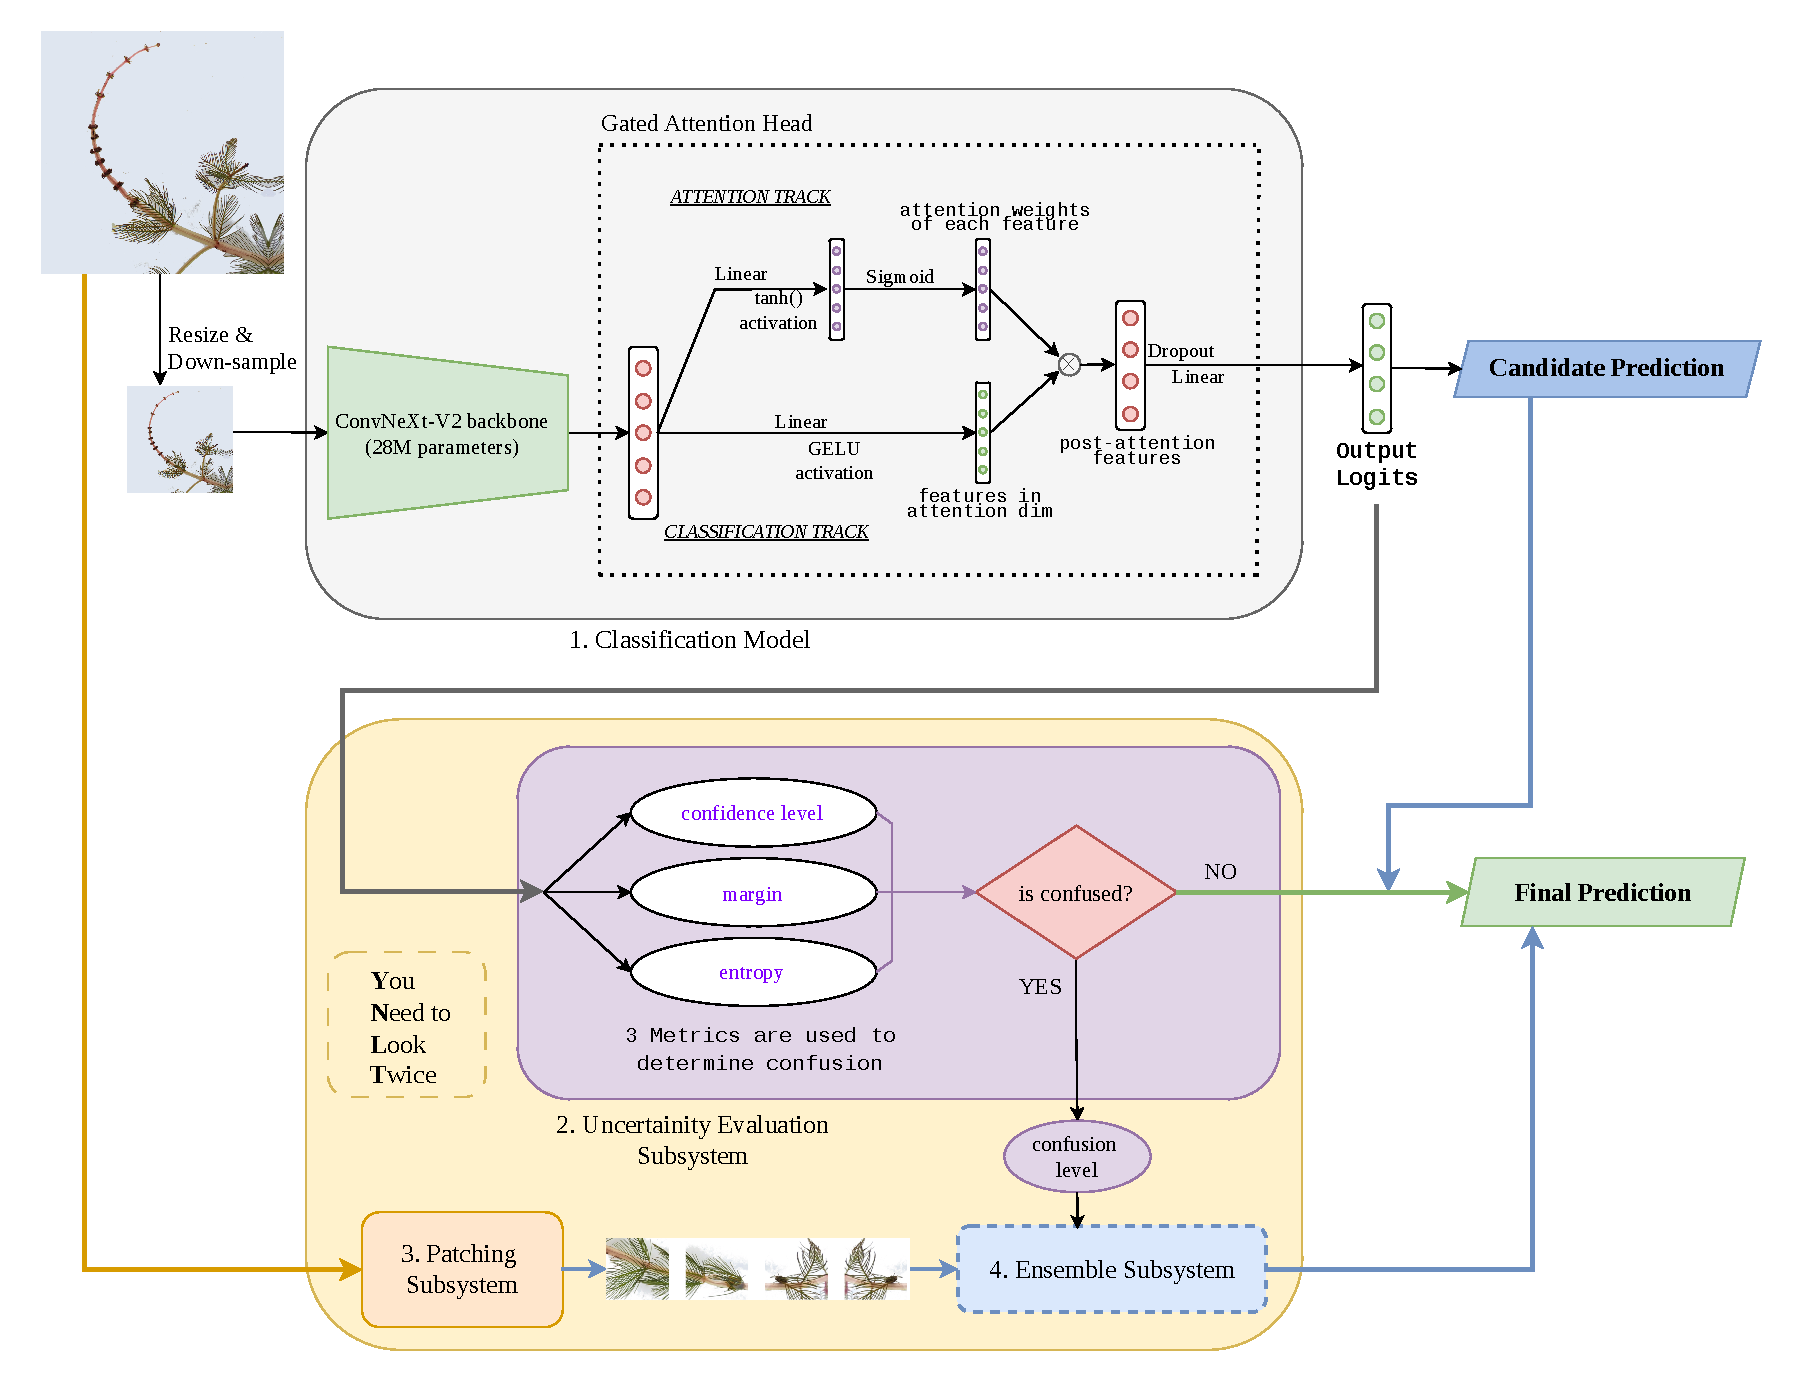
\includegraphics[width=1.0\textwidth]{figs/figs26/CombinedClassificatioAndConfusion_simplified.drawio.pdf}
\caption{Block diagram of the proposed Plant Species Classification pipeline. The system consists of two primary modules: (1) a feature extraction and classification network that outputs initial class logits, and (2) an uncertainty evaluation and ensembling system (YNLT) that assesses prediction confidence and re-evaluates the image using high-resolution patches if necessary.} 
\label{fig:model_block}
\end{figure*}

As illustrated in Figure \ref{fig:model_block}, the proposed architecture consists of two primary pathways. The first is the classification module, which processes an input image or patch to generate class-specific logits. The second module is the uncertainty evaluation system, which assesses the confidence of the initial prediction and, if necessary, triggers a high-resolution re-examination to finalize the classification.

\subsubsection{Pretrained ConvNeXt-V2 Backbone}

ConvNeXt-V2 integrates architectural choices studied for modern ConvNets~\citep{liu2022convnet} into a convolutional framework~\citep{Wooetal2023}. It incorporates mechanisms such as larger convolutional kernels and global response normalization (GRN) while retaining the spatial inductive biases characteristic of standard convolutional operations. This architecture provides high representational capacity without introducing the excessive parameter count typically associated with pure transformer models. Parameter efficiency is particularly critical for this study, as the limited training dataset significantly increases the risk of overfitting.

A primary advantage of utilizing ConvNeXt-V2 for this specific problem is its rigorous pretraining methodology. The model was pretrained using a Fully Convolutional Masked Autoencoder (FCMAE) framework \cite{Wooetal2023}, followed by supervised training on ImageNet-22k and final fine-tuning on ImageNet-1k. The ImageNet-22k dataset encompasses a vast hierarchical class structure, including several aquatic plant species within the same taxonomic families as those in the target dataset, such as pondweeds and waterlilies. Consequently, the pretrained backbone is used as a feature extractor for the 21 target species.

The Tiny variant was chosen with the deployment target in mind. An underwater rover carries an embedded computer whose GPU budget is shared with navigation, so the per-image cost of the backbone bounds the survey rate. On the RTX 3070 Ti used for these experiments, one \(224\times 224\) pass of ConvNeXt-V2 Tiny is 4.47~G multiply--adds and 5.2~ms. ResNet-50, measured on the same GPU with the same gated head, has 24.2~M parameters and 4.11~G multiply--adds and takes 3.6~ms per pass. The experiments in this paper use ConvNeXt-V2 Tiny.

\subsubsection{Model capacity and sample size}
\label{subsec:capacity}

In the head comparison only the classification head is trained, so the number of fitted weights is small compared with the 27.9~M frozen backbone weights: 16{,}149 for a linear head, 33{,}201 for a two-layer multilayer perceptron (MLP) with 42 hidden units, and 261{,}933 for the gated attention head of Section~\ref{subsec:gated}. The pooled training split contains about 650 images, which is still smaller than the gated head, so the classical heuristic of ten samples per free parameter is not met, and it is not the relevant yardstick. The head is a regularised probe on a fixed 768-dimensional representation. Weight decay, dropout, label smoothing, augmentation, and validation-based checkpoint selection bound its effective capacity. What governs such a probe is the number of examples per class, here on the order of 30 in the full training split. Section~\ref{subsec:curve} measures that relationship directly, training the linear and gated heads on 10\%, 25\%, 50\%, and 100\% of the training split. Section~\ref{subsec:heads} includes the MLP as an intermediate parameter count between the linear and gated heads. When the last ConvNeXt stage is trained (Section~\ref{subsec:laststage}), the trainable count rises to 15.5~M parameters.

\subsubsection{Gated Attention Classification Head}
\label{subsec:gated}

The ConvNeXt-V2 backbone extracts a global feature vector of length 768. A linear classifier maps these features directly to the 21 species. A gated head can reweight channels before that map. A standard multi-head self-attention module would add many more trainable parameters on a training split of a few hundred images, so it is not used.

To resolve this architectural trade-off, a parameter-efficient gated attention head was implemented, drawing on gated linear units~\citep{Dauphinetal2017} and query-dependent gating~\citep{Qiuetal2025}. Let \(h \in \mathbb{R}^{D}\) be the frozen backbone feature, with \(D=768\) for ConvNeXt-V2 Tiny, and let \(d=168\) be the bottleneck width. A classification branch and a gate branch are computed in parallel:

\[
u = \mathrm{GELU}(W_u h + b_u), \qquad
g = \sigma\bigl(\tanh(W_g h + b_g)\bigr),
\]
where \(\sigma\) is the logistic sigmoid and \(W_u, W_g \in \mathbb{R}^{d \times D}\)~\citep{HendrycksandGimpel2016}. The gated hidden state is the element-wise product \(u \odot g\), followed by dropout and a linear map to \(K=21\) logits. Only these head parameters (261{,}933 weights) are trained.

\subsection{You Need To Look Twice (YNLT) Module}

YNLT follows a simple rule: take a closer look only when the first look is unreliable. Many native and invasive aquatic plants are similar at low resolution and are distinguished by fine leaf or stem structure that is lost when a $3000\times 4000$ photograph is resized to $224\times 224$. Unlike always-on multi-crop testing~\citep{krizhevsky2012imagenet} or selective classifiers that abstain~\citep{geifman2017selective}, YNLT keeps the first prediction when it is confident and otherwise re-evaluates high-resolution patches of the original image.

\subsubsection{Uncertainty Evaluation Subsystem}

Let \(z \in \mathbb{R}^{K}\) be the head logits and
\[
p_i = \frac{e^{z_i}}{\sum_{j=1}^{K} e^{z_j}}, \qquad i=1,\ldots,K.
\]
Write \(p_{(1)}\ge p_{(2)}\ge \cdots \ge p_{(K)}\) for the sorted probabilities. Three scalar diagnostics are used~\citep{Guoetal2017, Ovadiaetal2019, hendrycks2017baseline}:

\[
\mathrm{Conf}(p) = p_{(1)}, \qquad
\mathrm{Marg}(p) = p_{(1)}-p_{(2)}, \qquad
H(p) = -\sum_{i=1}^{K} p_i \log p_i,
\]
where \(\log\) is the natural logarithm, matching the implementation. For \(K=21\), \(H(p)\) ranges from \(0\) (a point mass) to \(\log 21 \approx 3.04\) (the uniform distribution).

Each diagnostic contributes one count if it crosses a fixed threshold:

\[
\begin{aligned}
b_{\mathrm{conf}} &= \mathbf{1}\bigl[\mathrm{Conf}(p) < \tau_{\mathrm{conf}}\bigr], \\
b_{\mathrm{marg}} &= \mathbf{1}\bigl[\mathrm{Marg}(p) < \tau_{\mathrm{marg}}\bigr], \\
b_{\mathrm{ent}}  &= \mathbf{1}\bigl[H(p) > \tau_{H}\bigr], \\
c &= b_{\mathrm{conf}} + b_{\mathrm{marg}} + b_{\mathrm{ent}} \in \{0,1,2,3\}.
\end{aligned}
\]
The operating point used throughout this paper is \(\tau_{\mathrm{conf}}=0.5\), \(\tau_{\mathrm{marg}}=0.2\), \(\tau_{H}=2.0\). A first-pass prediction is sent to high-resolution review if \(c \ge \tau_{c}\) with \(\tau_{c}=1\), except when the predicted class is already invasive: in that case the invasive label is kept, so that YNLT cannot talk the model out of a positive detection.

\subsubsection{High-Resolution Patching Subsystem}
\label{subsec:patching}

When a prediction is flagged, the $224\times 224$ input is treated as insufficient and the image is re-examined at several scales. Patches are cut at relative scales \(s \in \{0.2, 0.3, 0.4, 0.5\}\) of the shorter side, with fractional overlaps \(\{0.0, 0.1, 0.2, 0.3\}\) respectively. Reflected padding is applied at each scale so that the stride tiles the image exactly, uniform patches (for example padding) are discarded, and every remaining patch is resized to $224\times 224$ and scored by the same frozen backbone and head. More scales and overlap improve coverage and increase the number of forward passes.

\paragraph{Patch source.} Which image the patches are cut from is a design choice in its own right. In the \emph{downsampled} setting the crops are taken from the $224\times 224$ network input, so the second look re-weights evidence the model has already seen; the schedule above yields 111 patches per reviewed image. In the \emph{full-resolution} setting the crops are taken from the original photograph, so the second look can recover detail that downsampling removed; a $1500\times 1000$ laboratory photograph yields 104 patches between 200 and 500 pixels wide, a $3000\times 4000$ one 99 patches between 600 and 1500 pixels. Both settings are implemented in the released code. All YNLT results in this paper use the downsampled source, which yields 111 patches per reviewed image.

\subsubsection{Ensemble Subsystem}

The Ensemble subsystem executes the actual ``second look" within the YNLT framework. It receives the collection of localized, high-resolution patches generated by the preceding subsystem and evaluates them to resolve the initial visual ambiguity. By shifting the model's focus from the downsampled global image to these detailed morphological features, the system gathers the precise evidence needed to make an informed final classification.

\begin{figure*}[!h]
  \centering
  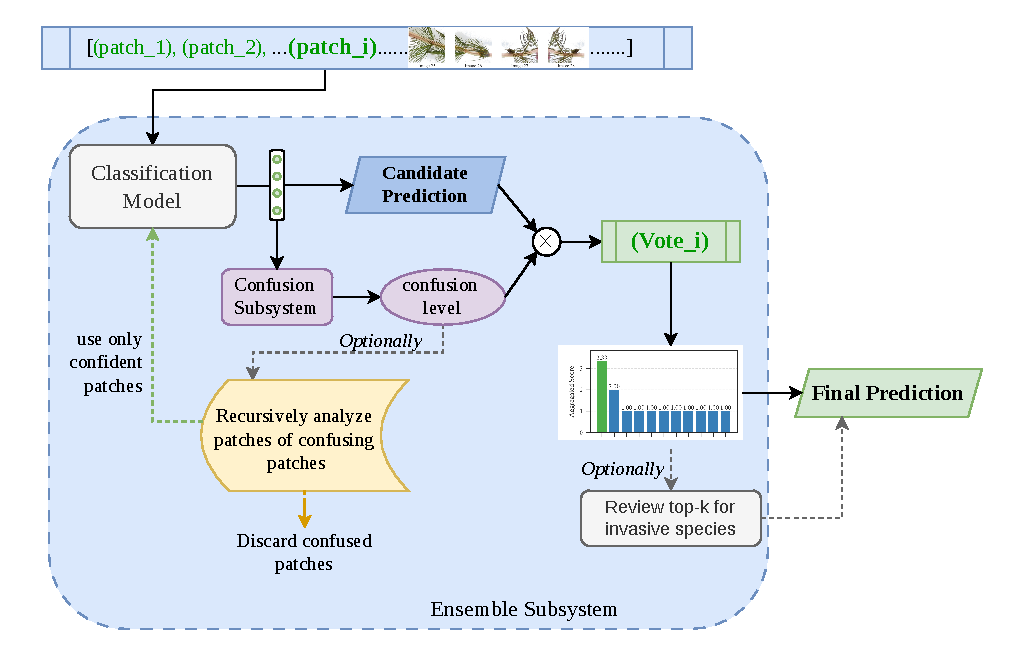
\includegraphics[width=1.0\textwidth]{figs/figs26/ensemble26_simplified.drawio.pdf}
  \caption{Workflow of the Ensemble subsystem. An image flagged for high uncertainty is divided into high-resolution patches. Each patch is processed independently by the classification pipeline and contributes a weighted vote to the final aggregated prediction.}
  \label{fig:ensemble}
\end{figure*}


Each patch is classified independently. Random-resized-crop training makes these partial views admissible inputs. Patch \(i\) with confusion count \(c_i\) contributes a normalized vote
\[
w_i = \frac{c_{\max}-c_i}{c_{\max}}, \qquad c_{\max}=3,
\]
to its predicted class. Accumulated class scores are initialized at \(1\) the first time a class appears, then incremented by \(w_i\). The class with the largest score is returned. If two classes share the maximum, an invasive class is preferred. This is a tie-break, not a top-\(k\) override: YNLT does not replace a unique non-invasive winner with an invasive runner-up.

\subsection{Evaluation Metrics}

During training, the primary indicators used to monitor model convergence were validation accuracy and loss. To prevent the network from generating overconfident predictions, which would compromise the YNLT module's ability to accurately detect uncertainty, label smoothing was applied in conjunction with standard cross-entropy. As demonstrated by \citet{Mulleretal2019}, label smoothing not only improves generalization but also significantly aids in model calibration by preventing the network from assigning full probability to the target class, thereby keeping the logits constrained. The smoothed cross-entropy loss is defined as:

\[
\mathcal{L}_{\text{smooth}} = - \sum_{i=1}^{K} q_i \log p_i
\]
where \( p_i \) is the predicted probability corresponding to class \( i \), \( K \) is the total number of classes, and the smoothed target distribution \( q_i \) is calculated as:

\[
 q_i = (1 - \epsilon) \delta_{i,y} + \frac{\epsilon}{K} 
\]
with \(\epsilon=0.05\) in the reported runs.

Overall model performance was evaluated using standard multi-class metrics, including overall accuracy and class-wise recall. However, given the ecological context of the study, predictions were also aggregated into a binary classification: Invasive (positive class) versus Native (negative class). In this binary framework, the most critical evaluation metric is the False Negative Rate (FNR). The ecological consequences of failing to identify an invasive species (a false negative) severely outweigh the operational costs of misclassifying a native plant as invasive (a false positive). Therefore, minimizing the FNR was a primary objective:
\[
\text{FNR} = \frac{\text{FN}}{\text{TP} + \text{FN}}
\]
where FN represents False Negatives and TP represents True Positives.

To specifically isolate and evaluate the utility of the proposed YNLT block, model predictions were tracked before and after the ensemble process. An image sent for review has one of four outcomes: a correct first prediction stays correct, a correct first prediction becomes incorrect, an incorrect first prediction becomes correct, or an incorrect first prediction stays incorrect.

Based on these transition cases, two custom metrics—Success Rate and Effectiveness—were defined to quantify the module's performance:

\[
\text{Success Rate} = \frac{\text{Total Correct After YNLT}}{\text{Total Images Reviewed by YNLT}}
\]

\[
\text{Effectiveness} = \frac{\text{Transitions from Incorrect to Correct}}{\text{Total Images Reviewed by YNLT}}
\]

These metrics served as key optimization targets for tuning the uncertainty thresholds, as well as the scale and overlap parameters within the patching subsystem.

\subsection{Experimentation}
\subsubsection{Training}
The model was implemented in PyTorch. The experiments in Sections~\ref{subsec:heads}--\ref{subsec:curve} were trained on an NVIDIA RTX 3070 Ti (8~GB) at batch size 32 with mixed precision. In the head comparison only the classification head was trained and the backbone remained frozen (27.9~M frozen parameters; 0.26~M trainable for the gated head). Measured at batch size 1 on that GPU, one \(224\times 224\) pass of ConvNeXt-V2 Tiny takes 5.2~ms (4.47~G multiply--adds, 28.1~M parameters). The same measurement for ResNet-50 is 3.6~ms (4.11~G multiply--adds, 24.2~M parameters). When YNLT reviews an image, about 111 patches are scored: about 209~ms for ConvNeXt-V2 Tiny and 129~ms for ResNet-50. These times are workstation measurements, not measurements on the rover's embedded computer. The experiments use ConvNeXt-V2 Tiny.

Training used AdamW~\citep{loshchilov2019adamw}, cosine learning-rate decay to \(2\times 10^{-5}\), 250 epochs, weight decay \(2\times 10^{-5}\), an initial learning rate of \(5\times 10^{-4}\), and label smoothing with \(\epsilon=0.05\)~\citep{szegedy2016rethinking, Mulleretal2019}. The checkpoint with the highest validation accuracy is kept. Each configuration is trained with five seeds (8--12). A seed changes the observation-level split and the initialisation of the head. In the last-stage experiment the last ConvNeXt stage is optimized at \(1\times 10^{-4}\) while the head keeps the learning rate above, and earlier stages stay frozen.

\subsubsection{Tuning YNLT Block}
YNLT trades accuracy against compute. The scales \(\{0.2,0.3,0.4,0.5\}\) and overlaps \(\{0.0,0.1,0.2,0.3\}\) were held fixed for the reported results. Recursion to still finer patches is implemented but disabled in the experiments here.

\section{Results}
\label{sec:results}

All numbers in this section are computed on the 1{,}030-image collection of Section~\ref{subsec:dataset}. Unless a single seed is named, each entry is the mean \(\pm\) standard deviation over seeds 8--12. Accuracy is 21-way top-1 accuracy. FNR is the invasive false-negative rate defined in Section~\ref{sec:materials_methods}.

\subsection{Classification head and YNLT}
\label{subsec:heads}

Table~\ref{tab:heads} compares the linear, MLP, and gated-attention heads on a frozen ConvNeXt-V2 Tiny encoder, with and without YNLT at test time. YNLT uses the downsampled patch source of Section~\ref{subsec:patching}. The laboratory and web columns are test-source metrics: they score the laboratory-origin and web-origin photographs that fell in the pooled test split. They are not a third category in Figure~\ref{fig:data}. The pooled column is the quantity used to compare models.

\begin{table*}[!ht]
    \caption{Accuracy and invasive false-negative rate of the linear, multilayer-perceptron, and gated-attention heads on a frozen ConvNeXt-V2 Tiny encoder, with and without YNLT, on the 1{,}030-image collection. Each entry is the mean \(\pm\) standard deviation over five seeds. Laboratory and web columns score laboratory-origin and web-origin images inside the pooled test; they are test-source metrics, not separate bars in Figure~\ref{fig:data}. The pooled columns are the mixed test used to compare the heads. YNLT uses the downsampled patch source.}
    \label{tab:heads}
    \renewcommand{\arraystretch}{1.25}
    \centering
    \small
    \begin{tabular}{lcccccc}
        \hline
        \multirow{2}{*}{\textbf{Head}} & \multicolumn{2}{c}{\textbf{Laboratory}} & \multicolumn{2}{c}{\textbf{Web}} & \multicolumn{2}{c}{\textbf{Pooled}} \\
        \cline{2-3} \cline{4-5} \cline{6-7}
        & \textbf{Acc.} & \textbf{FNR} & \textbf{Acc.} & \textbf{FNR} & \textbf{Acc.} & \textbf{FNR} \\
        \hline
        Linear & 80.0 $\pm$ 8.0 & 15.6 $\pm$ 9.9 & 53.0 $\pm$ 4.7 & 35.4 $\pm$ 9.9 & 59.5 $\pm$ 4.6 & 31.3 $\pm$ 7.6 \\
        Linear + YNLT & 75.9 $\pm$ 7.2 & 6.7 $\pm$ 9.9 & 50.9 $\pm$ 2.8 & 25.7 $\pm$ 9.4 & 57.1 $\pm$ 2.6 & 22.2 $\pm$ 6.9 \\
        MLP & 77.4 $\pm$ 10.0 & 11.1 $\pm$ 13.6 & 53.7 $\pm$ 3.5 & 32.6 $\pm$ 5.8 & 59.4 $\pm$ 4.3 & 28.4 $\pm$ 5.5 \\
        MLP + YNLT & 77.4 $\pm$ 11.2 & 6.7 $\pm$ 9.9 & 52.5 $\pm$ 2.7 & 20.7 $\pm$ 6.8 & 58.5 $\pm$ 3.6 & 18.4 $\pm$ 4.4 \\
        Gated attention & 80.0 $\pm$ 5.8 & 8.9 $\pm$ 9.3 & 52.0 $\pm$ 5.2 & 37.6 $\pm$ 6.5 & 58.6 $\pm$ 4.6 & 32.6 $\pm$ 3.9 \\
        Gated attention + YNLT & 79.0 $\pm$ 7.6 & 2.2 $\pm$ 5.0 & 52.5 $\pm$ 3.8 & 19.9 $\pm$ 5.7 & 58.8 $\pm$ 4.0 & 17.4 $\pm$ 5.7 \\
        \hline
    \end{tabular}
\end{table*}

On pooled accuracy the three heads agree. The linear head reaches \(59.5\% \pm 4.6\%\), the MLP \(59.4\% \pm 4.3\%\), and gated attention \(58.6\% \pm 4.6\%\). Each difference is smaller than the seed-to-seed standard deviation, so the extra weights in the gated head do not change 21-way accuracy on this collection. Laboratory-origin accuracy is higher than web-origin accuracy for every head (about 80\% against about 52--54\%), which is consistent with the simpler backgrounds in the laboratory photographs. The locally collected outdoor photographs contribute only about eight images to a given pooled test split. Accuracy on that slice falls between 70\% and 75\%, with standard deviations of 7 to 15 points, and it is not used to rank models.

YNLT changes the invasive FNR more than it changes accuracy. For the gated head, pooled accuracy moves from \(58.6\% \pm 4.6\%\) to \(58.8\% \pm 4.0\%\), while the pooled invasive FNR falls from \(32.6\% \pm 3.9\%\) to \(17.4\% \pm 5.7\%\). The linear head shows the same pattern: pooled accuracy falls from \(59.5\% \pm 4.6\%\) to \(57.1\% \pm 2.6\%\), and the pooled FNR falls from \(31.3\% \pm 7.6\%\) to \(22.2\% \pm 6.9\%\). The FNR reduction is larger than the accuracy change, and for the gated head it exceeds the standard deviation of the frozen-head FNR.

\subsection{Training the last ConvNeXt stage}
\label{subsec:laststage}

Table~\ref{tab:laststage} keeps the linear head, the augmentation schedule, and the 1{,}030-image collection, and trains the last ConvNeXt-V2 stage at a learning rate of \(1\times 10^{-4}\). Earlier stages stay frozen. The checkpoint remains the epoch of highest validation accuracy.

\begin{table*}[!ht]
    \centering
    \caption{Linear head on the 1{,}030-image collection, five seeds. The second row trains the last ConvNeXt-V2 stage. Accuracy and invasive FNR are percentages, mean \(\pm\) standard deviation.}
    \label{tab:laststage}
    \renewcommand{\arraystretch}{1.2}
    \small
    \begin{tabular}{lcccc}
        \hline
        \textbf{Encoder} & \textbf{Pooled acc.} & \textbf{Laboratory acc.} & \textbf{Web acc.} & \textbf{Pooled FNR} \\
        \hline
        Frozen & 59.5 $\pm$ 4.6 & 80.0 $\pm$ 8.0 & 53.0 $\pm$ 4.7 & 31.3 $\pm$ 7.6 \\
        Last stage trained & 65.1 $\pm$ 5.0 & 85.6 $\pm$ 9.7 & 58.1 $\pm$ 4.8 & 28.8 $\pm$ 9.6 \\
        \hline
    \end{tabular}
\end{table*}

Pooled accuracy rises from \(59.5\% \pm 4.6\%\) to \(65.1\% \pm 5.0\%\), a gain of about five points on both the laboratory-origin and web-origin portions of the test. The invasive FNR moves from \(31.3\% \pm 7.6\%\) to \(28.8\% \pm 9.6\%\). That change is smaller than the standard deviation, so it is not evidence that the last stage improves invasive detection. Among the settings trained on this collection, the last-stage linear model has the highest pooled accuracy. The lowest pooled invasive FNR remains the frozen gated head with YNLT (Table~\ref{tab:heads}).

\subsection{Learning curve}
\label{subsec:curve}

Figure~\ref{fig:curve} plots test accuracy against the number of training images for the linear and gated heads. Fractions of 10\%, 25\%, 50\%, and 100\% of the pooled training split were used, with whole observations kept together and at least one observation per species. The validation and test splits were held fixed. The 10--50\% points use three seeds, and the 100\% point uses the five seeds of Table~\ref{tab:heads}. YNLT is not applied.

\begin{figure*}[!ht]
  \centering
  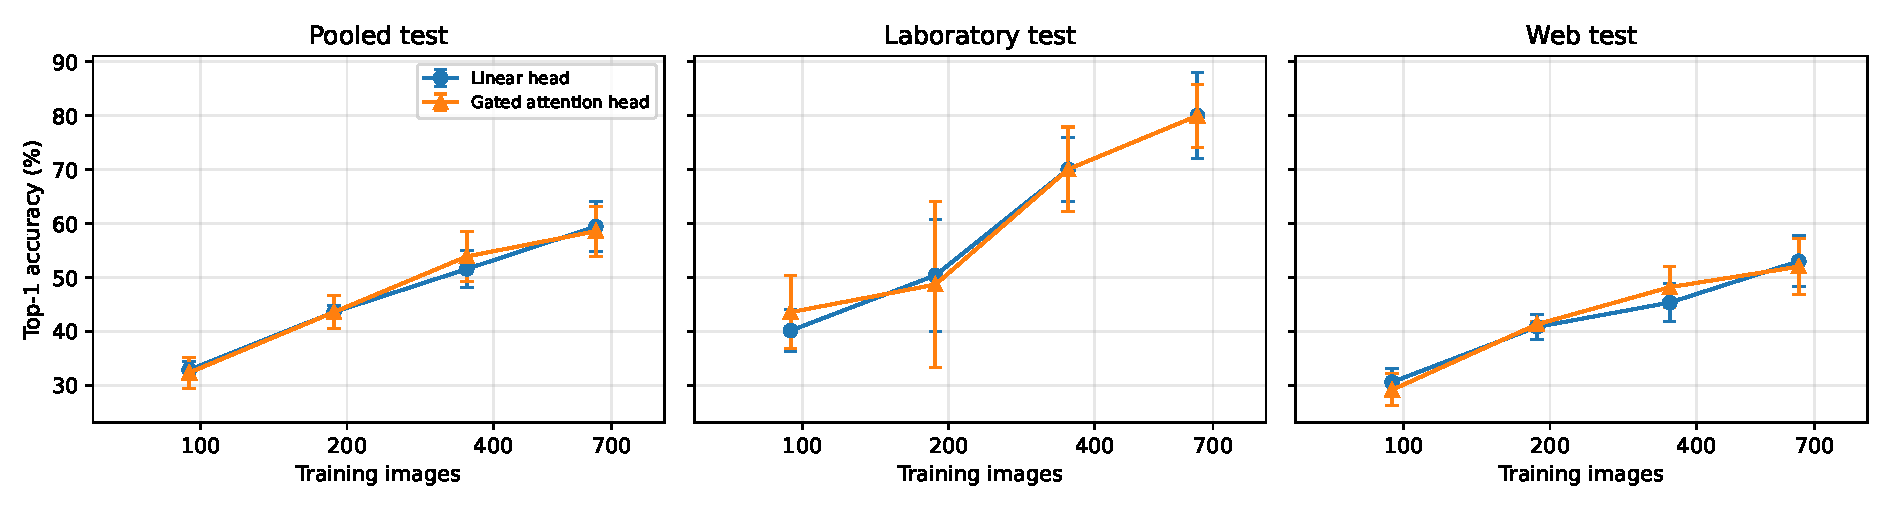
\includegraphics[width=1.0\textwidth]{figs/learning_curve.pdf}
  \caption{Top-1 accuracy against the number of training images for the linear and gated-attention heads on a frozen ConvNeXt-V2 Tiny encoder. Mean \(\pm\) standard deviation; three seeds at the smaller fractions and five seeds at the full split. YNLT is not applied.}
  \label{fig:curve}
\end{figure*}

On the pooled test, linear-head accuracy rises from \(32.9\% \pm 1.6\%\) at 95 training images to \(43.6\% \pm 1.2\%\) at 188, \(51.6\% \pm 3.5\%\) at 353, and \(59.5\% \pm 4.6\%\) at 650. The gated head follows the same path, from \(32.4\% \pm 2.9\%\) to \(58.6\% \pm 4.6\%\). Neither curve has flattened. The laboratory-origin panel rises from about 40\% to \(80.0\%\), and the web-origin panel from about 30\% to \(52\)--\(53\%\). Additional photographs of the same kind would still be expected to raise accuracy. The gated head is not more data-hungry than the linear head, which matches the capacity argument of Section~\ref{subsec:capacity}.

\subsection{Training and validation loss}
\label{subsec:loss}

Figure~\ref{fig:loss} shows the mean training and validation loss for the three frozen heads. For each head the mean validation loss falls during the early epochs and then stays near 1.5 through epoch 250, while the training loss continues to decline slowly under augmentation and label smoothing. The saved checkpoint is the epoch of highest validation accuracy, which lies on that plateau.

\begin{figure*}[!ht]
  \centering
  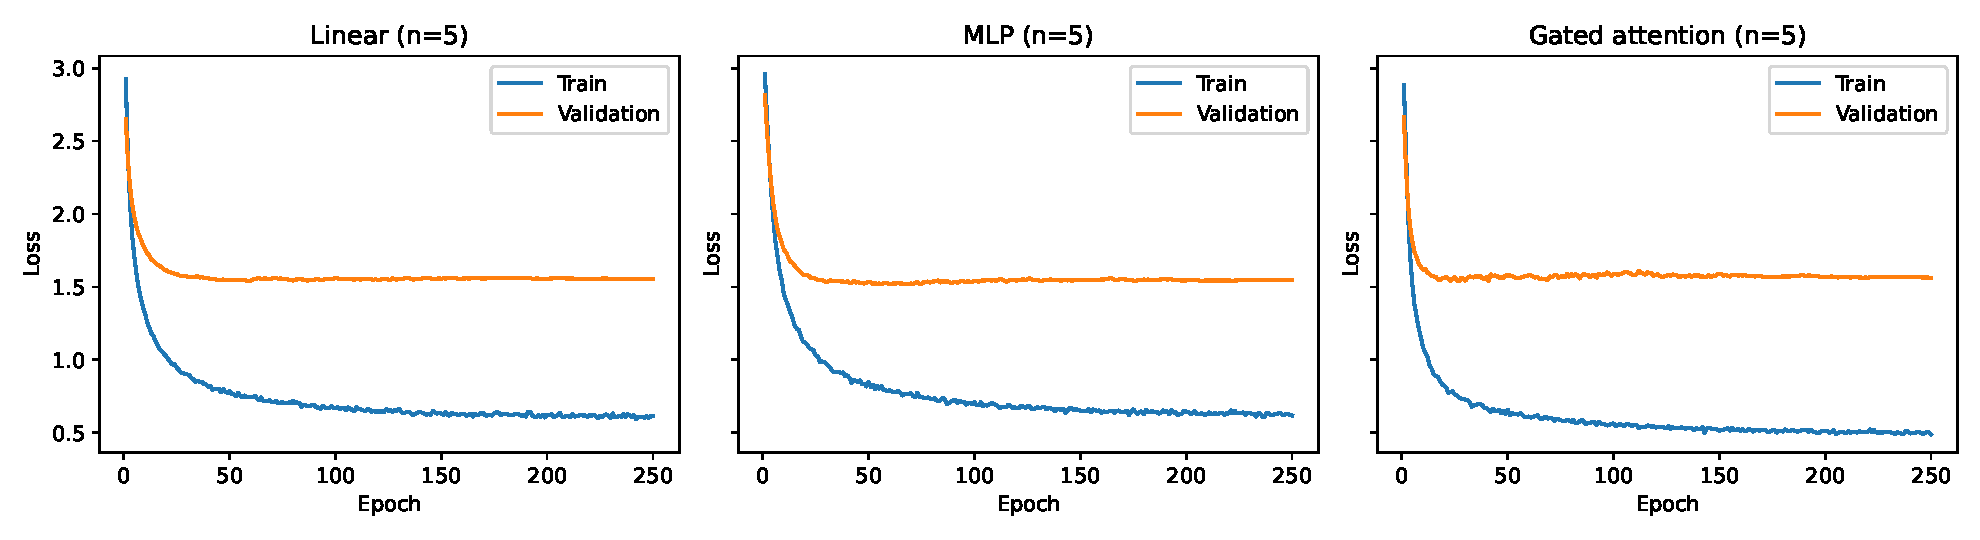
\includegraphics[width=1.0\textwidth]{figs/loss_curves.pdf}
  \caption{Mean training and validation loss over five seeds for each frozen head on the 1{,}030-image collection. The checkpoint is the epoch of highest validation accuracy.}
  \label{fig:loss}
\end{figure*}

\subsection{Species-level errors and class activation maps}
\label{subsec:errors}

The species-level counts below are for one checkpoint: the frozen linear head, seed 9, scored on its pooled test of 189 images. That checkpoint classifies 126 images correctly (66.7\%). Nine of 48 invasive test images are missed, an invasive FNR of 18.8\% on this split. These counts illustrate where errors fall. They are not the five-seed means of Tables~\ref{tab:heads} and~\ref{tab:laststage}.

\begin{table*}[!ht]
    \centering
    \caption{Per-species recall of the frozen linear head, seed 9, on its pooled test of 189 images (126 correct, 66.7\%). Invasive species are marked with an asterisk. These counts are for one checkpoint and are not the five-seed means in Tables~\ref{tab:heads} and~\ref{tab:laststage}.}
    \label{tab:recall}
    \renewcommand{\arraystretch}{1.05}
    \small
    \begin{tabular}{lrrr}
        \hline
        \textbf{Species} & \textbf{Test images} & \textbf{Correct} & \textbf{Recall (\%)} \\
        \hline
        Brasenia schreberi & 9 & 7 & 78 \\
        Cabomba$^{*}$ & 9 & 8 & 89 \\
        Ceratophyllum demersum & 9 & 7 & 78 \\
        Elodea canadensis & 3 & 2 & 67 \\
        Heteranthera dubia & 6 & 5 & 83 \\
        Hydrocharis morsus-ranae$^{*}$ & 6 & 6 & 100 \\
        Myriophyllum sibiricum & 6 & 3 & 50 \\
        Myriophyllum spicatum$^{*}$ & 10 & 6 & 60 \\
        Najas flexilis & 4 & 3 & 75 \\
        Nitellopsis obtusa$^{*}$ & 9 & 6 & 67 \\
        Nuphar variegata & 11 & 9 & 82 \\
        Nymphaea odorata & 7 & 5 & 71 \\
        Potamogeton crispus$^{*}$ & 14 & 6 & 43 \\
        Potamogeton gramineus & 24 & 13 & 54 \\
        Potamogeton illinoensis & 12 & 8 & 67 \\
        Potamogeton natans & 7 & 5 & 71 \\
        Potamogeton praelongus & 10 & 2 & 20 \\
        Potamogeton richardsonii & 7 & 2 & 29 \\
        Potamogeton robbinsii & 5 & 5 & 100 \\
        Ranunculus aquatilis & 13 & 13 & 100 \\
        Vallisneria americana & 8 & 5 & 62 \\
        \hline
    \end{tabular}
\end{table*}

Table~\ref{tab:recall} shows that recall is uneven. \emph{Hydrocharis morsus-ranae}, \emph{Potamogeton robbinsii}, and \emph{Ranunculus aquatilis} are correct on every test image of this split. The lowest recalls are \emph{Potamogeton praelongus} (2 of 10), \emph{Potamogeton richardsonii} (2 of 7), and \emph{Potamogeton crispus} (6 of 14). Of the 63 mistakes, 28 (44\%) stay inside the same genus. The most frequent pair is \emph{Potamogeton praelongus} predicted as \emph{Potamogeton crispus} (4 images). \emph{Myriophyllum spicatum} is predicted as \emph{Cabomba} twice. The remaining cross-genus mistakes are mostly between plants that share a growth form, either finely divided submerged leaves or broad floating leaves.

\begin{figure*}[!ht]
  \centering
  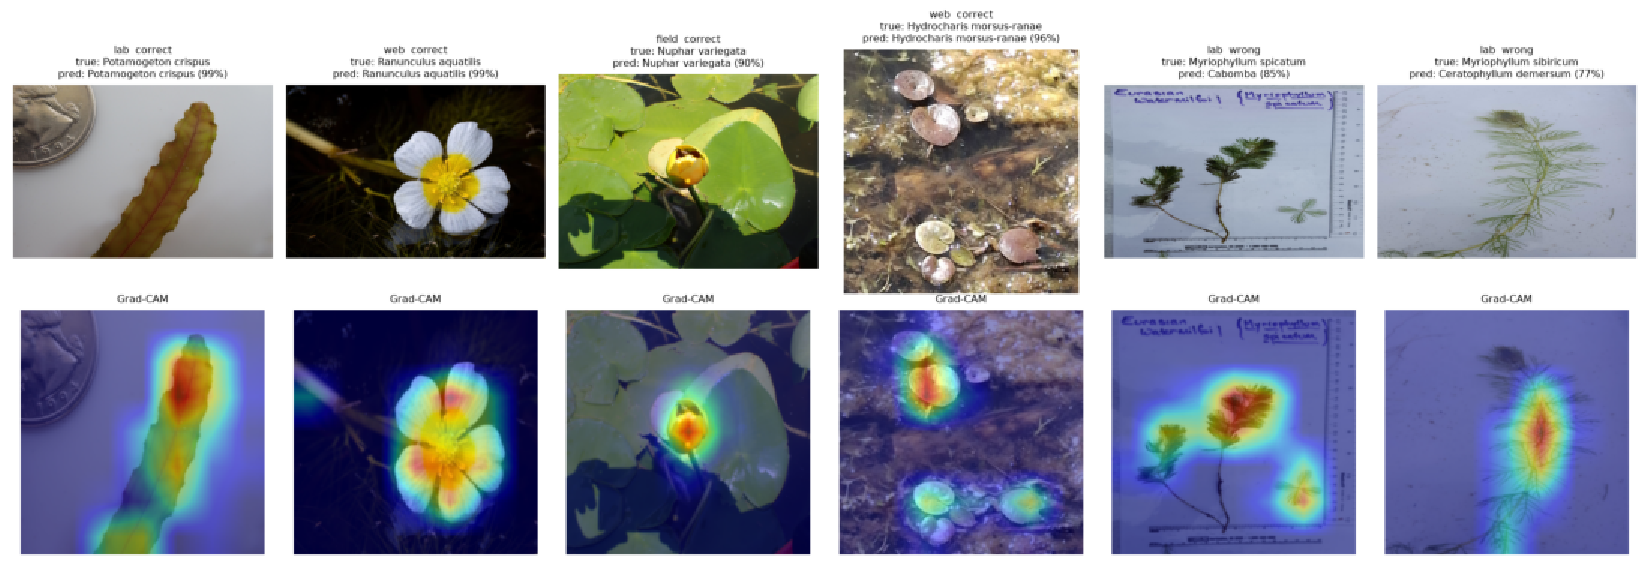
\includegraphics[width=1.0\textwidth]{figs/gradcam_panel.pdf}
  \caption{Gradient-weighted class activation maps~\citep{selvaraju2017gradcam} for the frozen linear head, seed 9. Each pair shows the network input and the map for the predicted class. Correct examples attend to the plant rather than to a coin, a label, or open water. Incorrect examples also attend to foliage, including look-alike species.}
  \label{fig:gradcam}
\end{figure*}

Figure~\ref{fig:gradcam} applies Grad-CAM at the last ConvNeXt stage of the same seed-9 checkpoint. On correct laboratory and outdoor photographs the highest weights lie on the leaf, flower, or floating blade, including when a coin or a handwritten label is in the frame. On the two incorrect examples the map still lies on the foliage. The error is a confusion between similar plants, not a response to the background.

\section{Discussion}

\textbf{What the 1{,}030-image collection supports.}
The reported classifier is trained and tested on one mixed collection of 203 laboratory photographs and 827 outdoor photographs. Handheld photographs were removed and are not part of the evaluation. The results therefore describe identification within this collection. They do not measure performance on underwater rover imagery. That imagery remains future data.

\textbf{Head, second look, and the last encoder stage.}
With the encoder frozen, pooled accuracy does not separate the linear, MLP, and gated heads (Table~\ref{tab:heads}). The gated head is retained as an option because, together with YNLT, it gives the lowest invasive FNR in that table (\(17.4\% \pm 5.7\%\)). YNLT spends the extra forward passes only when the first prediction is uncertain, which is the intended behavior, and the accuracy cost on the pooled test is about two points or less. Training the last ConvNeXt stage raises pooled accuracy by about five points (Table~\ref{tab:laststage}) without a clear change in invasive FNR. The two results answer different questions: last-stage training for 21-way accuracy, and YNLT for missed invasive species.

\textbf{Where the remaining errors are.}
The learning curve is still rising at about 650 training images (Figure~\ref{fig:curve}), so more photographs would still be expected to help. The species counts say which photographs. Errors concentrate on \emph{Potamogeton praelongus}, \emph{Potamogeton crispus}, and \emph{Potamogeton richardsonii}, and on feathery species that share a growth form with \emph{Cabomba}. Grad-CAM indicates that these mistakes are not explained by the model ignoring the plant. Adding photographs of those taxa is a more direct next step than changing the head.

\textbf{Sample size and fitted weights.}
On the frozen encoder, 16{,}149 to 261{,}933 head weights are fit to a 768-dimensional vector. Figure~\ref{fig:curve} shows that the gated head, with sixteen times the weights of the linear head, matches the linear head at every training size that was tried. The number of images per class, not the width of the head, is what moves accuracy. The five-seed standard deviations are several points on the pooled test and larger on the laboratory slice, so differences smaller than that spread are not interpreted as improvements.

\textbf{Computation.}
A frozen ConvNeXt-V2 Tiny encoder plus the gated head contains 28.1~M parameters, of which 0.26~M are trained. One \(224\times 224\) forward pass is 4.47~G multiply--adds and 5.2~ms on the RTX 3070 Ti. YNLT adds about 111 forward passes, or about 209~ms, for each reviewed image. On the same GPU, ResNet-50 takes 3.6~ms per pass and 129~ms per review. Training the last ConvNeXt stage raises the trainable count to 15.5~M and does not change the inference cost of a single pass. Latency on the rover's embedded computer has not been measured. Until it is, the demonstrated operating point is the workstation used here.

\textbf{Limitations.}
Several species still have only a few laboratory photographs, and \emph{Elodea canadensis} has no outdoor photographs after cleaning. Most outdoor photographs are GBIF field images, geographically uneven, and many carry licences that allow research use but not redistribution. Only 42 of the 827 outdoor photographs are locally collected, and only about eight of those fall in a given test split. Grad-CAM and the per-species recalls are reported for one seed of the frozen linear model, so they should be read as an error analysis of that checkpoint, not as a five-seed estimate. A biology-specific encoder was not trained. Underwater video from the rover is not in the collection.

\textbf{Use of the model.}
On a workstation, the model can screen photographs of these 21 species before a botanist confirms the record. The invasive FNR, rather than top-1 accuracy alone, is the quantity that should be watched for that use. Onboard screening on an underwater rover requires a measured latency budget and photographs from that camera. Neither is part of the present evaluation.

\section{Conclusion}
\label{sec:conclu}

This study classifies 21 Michigan aquatic plant species, five of them invasive, from a mixed collection of 1{,}030 photographs. The collection combines 203 laboratory photographs and 827 outdoor photographs. The outdoor total includes cleaned GBIF photographs and 42 locally collected outdoor photographs. Handheld photographs are excluded, and photographs from the same observation stay in one split.

With a frozen ConvNeXt-V2 Tiny encoder, a linear head, an MLP, and a gated-attention head reach \(58.6\%\) to \(59.5\%\) pooled top-1 accuracy over five seeds. The differences are smaller than the seed-to-seed spread. YNLT, which re-evaluates an image only when the first prediction is uncertain, lowers the pooled invasive FNR of the gated head from \(32.6\% \pm 3.9\%\) to \(17.4\% \pm 5.7\%\). Training the last ConvNeXt stage raises pooled accuracy from \(59.5\% \pm 4.6\%\) to \(65.1\% \pm 5.0\%\) and does not clearly change the invasive FNR. Accuracy is still increasing at about 650 training images. The mistakes that remain are concentrated on look-alike pondweeds, and class activation maps place the network's response on the plant rather than on the background. Inference cost on the rover's computer, and photographs from that camera, are the remaining steps before onboard use.


\section*{Authorship Contribution}

\textbf{Aaryan Panigrahi}: Formal analysis, Software, Writing - original draft; \\
\textbf{Fengying Dang}: Conceptualization, Investigation, Data curation, Supervision, Writing - original \& draft \& review \& editing.  

\section*{Acknowledgement}
The authors thank Dr. Jo Latimore for providing the weed images that supported the experimental evaluation.

% This work was supported in part by ???. 
% helping annotate the weed images and Dr. ??? for the assistance in weed identification. 

\typeout{}
% \bibliographystyle{model1-num-names}
\bibliography{ref}
\end{document}

